\documentclass[fleqn]{article}

\usepackage{polski}
\usepackage[utf8]{inputenc}
\usepackage[polish]{babel}
\usepackage{parskip}
\usepackage{icomma}
\usepackage[a4paper,includeheadfoot,margin=2.54cm]{geometry}
\usepackage{svg}
\usepackage{float}
\usepackage{graphicx}
\usepackage{amsmath}
\usepackage{subcaption}

\renewcommand\thesection{\arabic{section}.}
\renewcommand\thesubsection{\arabic{section}. \alph{subsection})}
\renewcommand\thesubsubsection{}

\brokenpenalty=1000
\clubpenalty=1000
\widowpenalty=1000

\title{TM -- Laboratorium 1.}
\author{Krystian Chachuła \\ Dawid Gruszczyński \\ Marcin Skrzypkowski}

\begin{document}

\maketitle

\setcounter{page}{0}
\thispagestyle{empty}

\pagebreak

\setcounter{page}{1}

\section{} % TODO: tu wstawić nazwę pierwszego zadania

Lorem ipsum dolor sit amet, consectetur adipiscing elit. Pellentesque gravida, est non consectetur dapibus, mauris massa pretium tortor, ut congue ex ligula at ante. Praesent blandit risus eu quam mattis, eu vulputate ante luctus. Etiam vitae quam justo. In sit amet hendrerit velit, non feugiat enim. In sit amet porttitor justo. Orci varius natoque penatibus et magnis dis parturient montes, nascetur ridiculus mus. Suspendisse potenti. Morbi facilisis lectus venenatis mauris lacinia, in aliquet ligula semper. Ut placerat, mauris at hendrerit consequat, eros odio efficitur nisl, non fringilla lorem nisl ac diam. Donec eget egestas dui. Sed ultricies pulvinar eros, sit amet ultrices mauris efficitur ut. Donec at ligula pretium, varius diam eu, aliquet urna. Quisque condimentum, nulla iaculis pharetra cursus, purus felis posuere tellus, quis interdum ante velit vel libero. Donec eget egestas ante. In posuere odio nec libero dignissim, a mollis felis laoreet.

\begin{figure}[H]
	\centering
	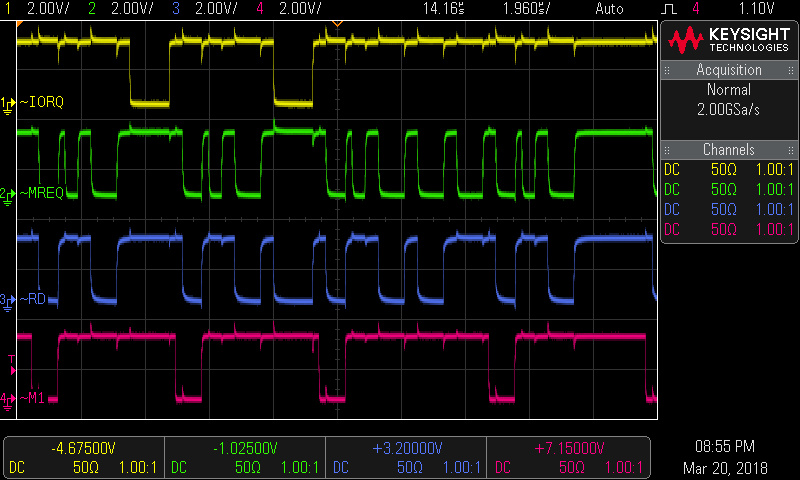
\includegraphics[width=0.75\textwidth]{img/1a.png}
	\caption{}
\end{figure}

\section{} % TODO: tu wstawić nazwę drugiego zadania

\begin{figure}[H]
	\centering
	\begin{subfigure}[b]{0.49\textwidth}
		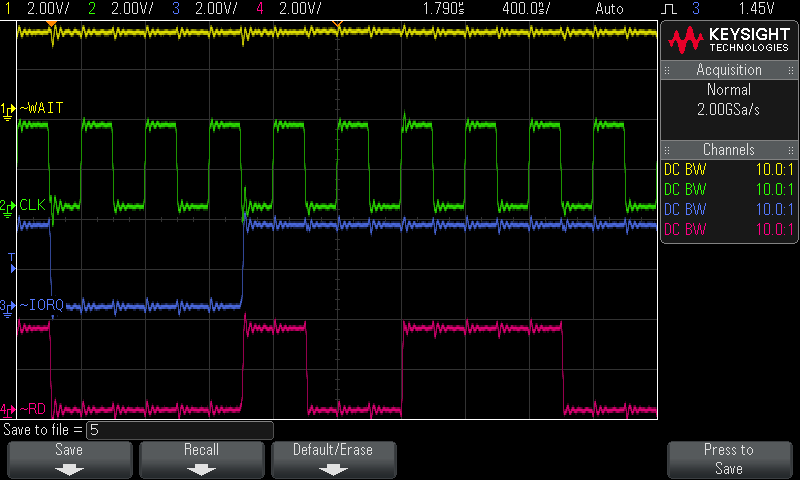
\includegraphics[width=\textwidth]{img/2a.png}
		\caption{}
	\end{subfigure}
	\begin{subfigure}[b]{0.49\textwidth}
		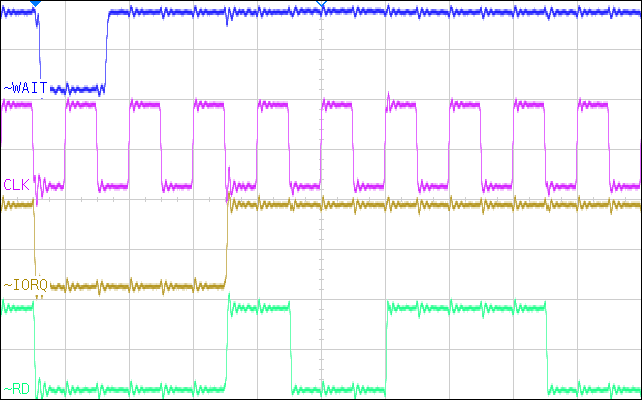
\includegraphics[width=\textwidth]{img/2b.png}
		\caption{}
	\end{subfigure}
	\begin{subfigure}[b]{0.49\textwidth}
		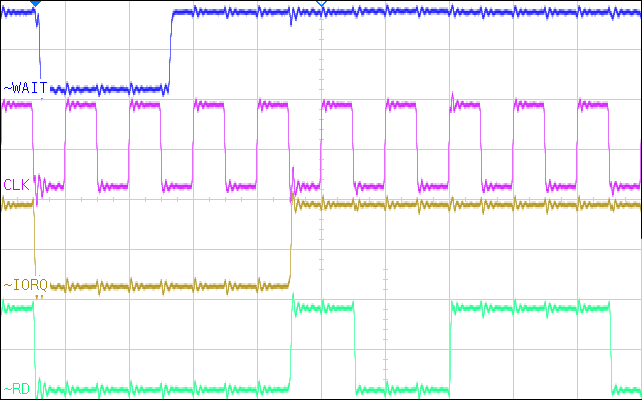
\includegraphics[width=\textwidth]{img/2c.png}
		\caption{}
	\end{subfigure}
	\begin{subfigure}[b]{0.49\textwidth}
		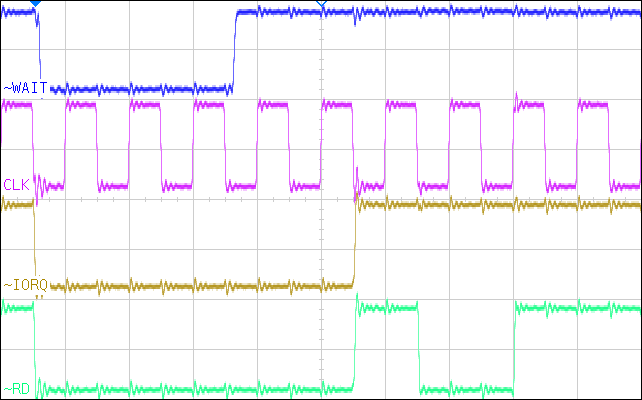
\includegraphics[width=\textwidth]{img/2d.png}
		\caption{}
	\end{subfigure}
	\begin{subfigure}[b]{0.49\textwidth}
		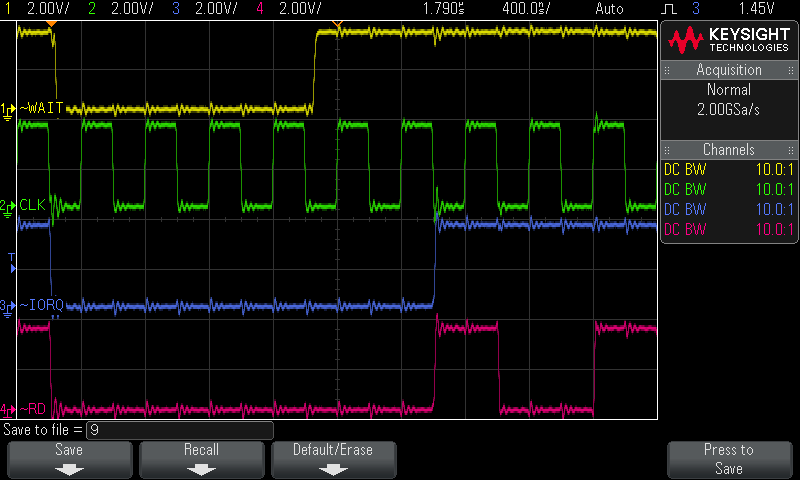
\includegraphics[width=\textwidth]{img/2e.png}
		\caption{}
	\end{subfigure}
	\caption{}
\end{figure}

\section{} % TODO: tu wstawić nazwę trzeciego zadania

\begin{figure}[H]
	\centering
	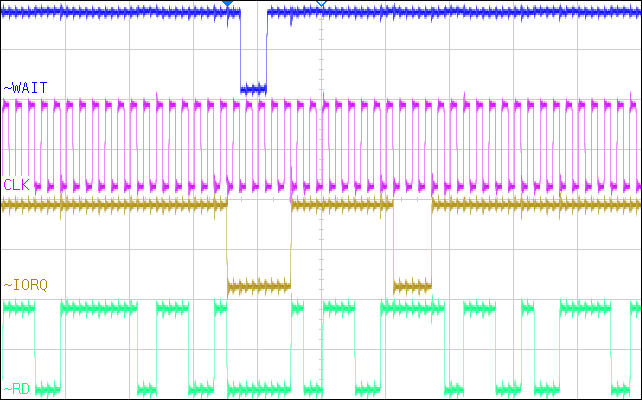
\includegraphics[width=0.75\textwidth]{img/3a.png}
	\caption{}
\end{figure}

\begin{figure}[H]
	\centering
	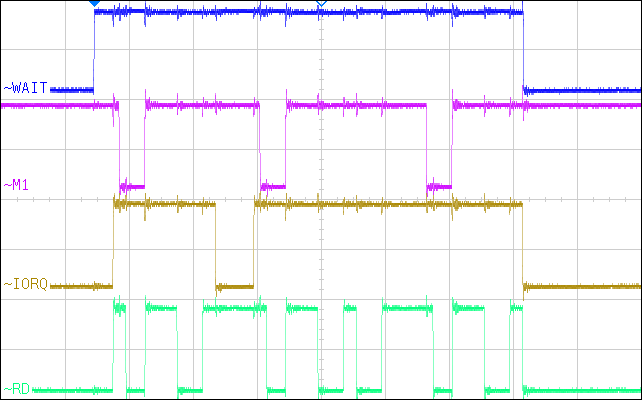
\includegraphics[width=0.75\textwidth]{img/3b.png}
	\caption{}
\end{figure}

\begin{figure}[H]
	\centering
	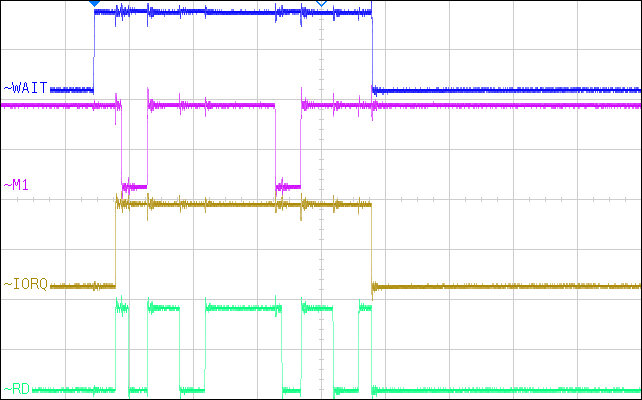
\includegraphics[width=0.75\textwidth]{img/3c.png}
	\caption{}
\end{figure}

\end{document}
